\documentclass{article}

\usepackage[normalem]{ulem}
\usepackage[margin=1in]{geometry}
\usepackage{enumitem}

\usepackage{float}
\usepackage{graphicx}
\graphicspath{{./}}

\usepackage{fancyhdr}
\pagestyle{fancy}

\usepackage{hyperref}

\newcommand{\Team}{null'); DROP TABLE Students;}

\lhead{\Team}
\chead{\Large \textbf{Phase 1}\vspace{0pt}}
\rhead{\today}
\setlength{\headheight}{46pt}
\setlength{\headsep}{4ex}

\renewcommand{\arraystretch}{1.3}
\setlist[itemize, 2]{label={--}}


\title{Principles of Data Management\\\Large Phase 2\\\vspace{14pt}\Team}
\date{\today}
\author{
	Andrew Hamrick
	\and
	Daniyal Iqbal
	\and
	Oscar Lowry
	\and
	Qasim Ali
}

\begin{document}
	\maketitle
  \thispagestyle{empty}
	\newpage

	\section{Design}
		Our database was designed with a Retail environment in mind. The choices for
		entities and relations were made by considering what retail employees and
		stores would likely need to check or keep track of. The retail environment
		envisioned focuses on electronic devices. Currently our design supports
		Computers and TVs but can easily be expanded to other product types. We
		decided to focus on computers and TVs as that is an area of expertise for
		us.\\
		\vspace{0pt}

		Our database centers around the product entity as that is largely seen as
		the most important component of a retail environment. The other entities
		were chosen to track the flow of money in and out of the stores, or to
		support the product. Support for the products includes keeping track of
		current inventory, acquiring more of the product, and categorizing the
		product into product types.

	\section{ER Diagram}
    \begin{figure}[H]
      \centering
      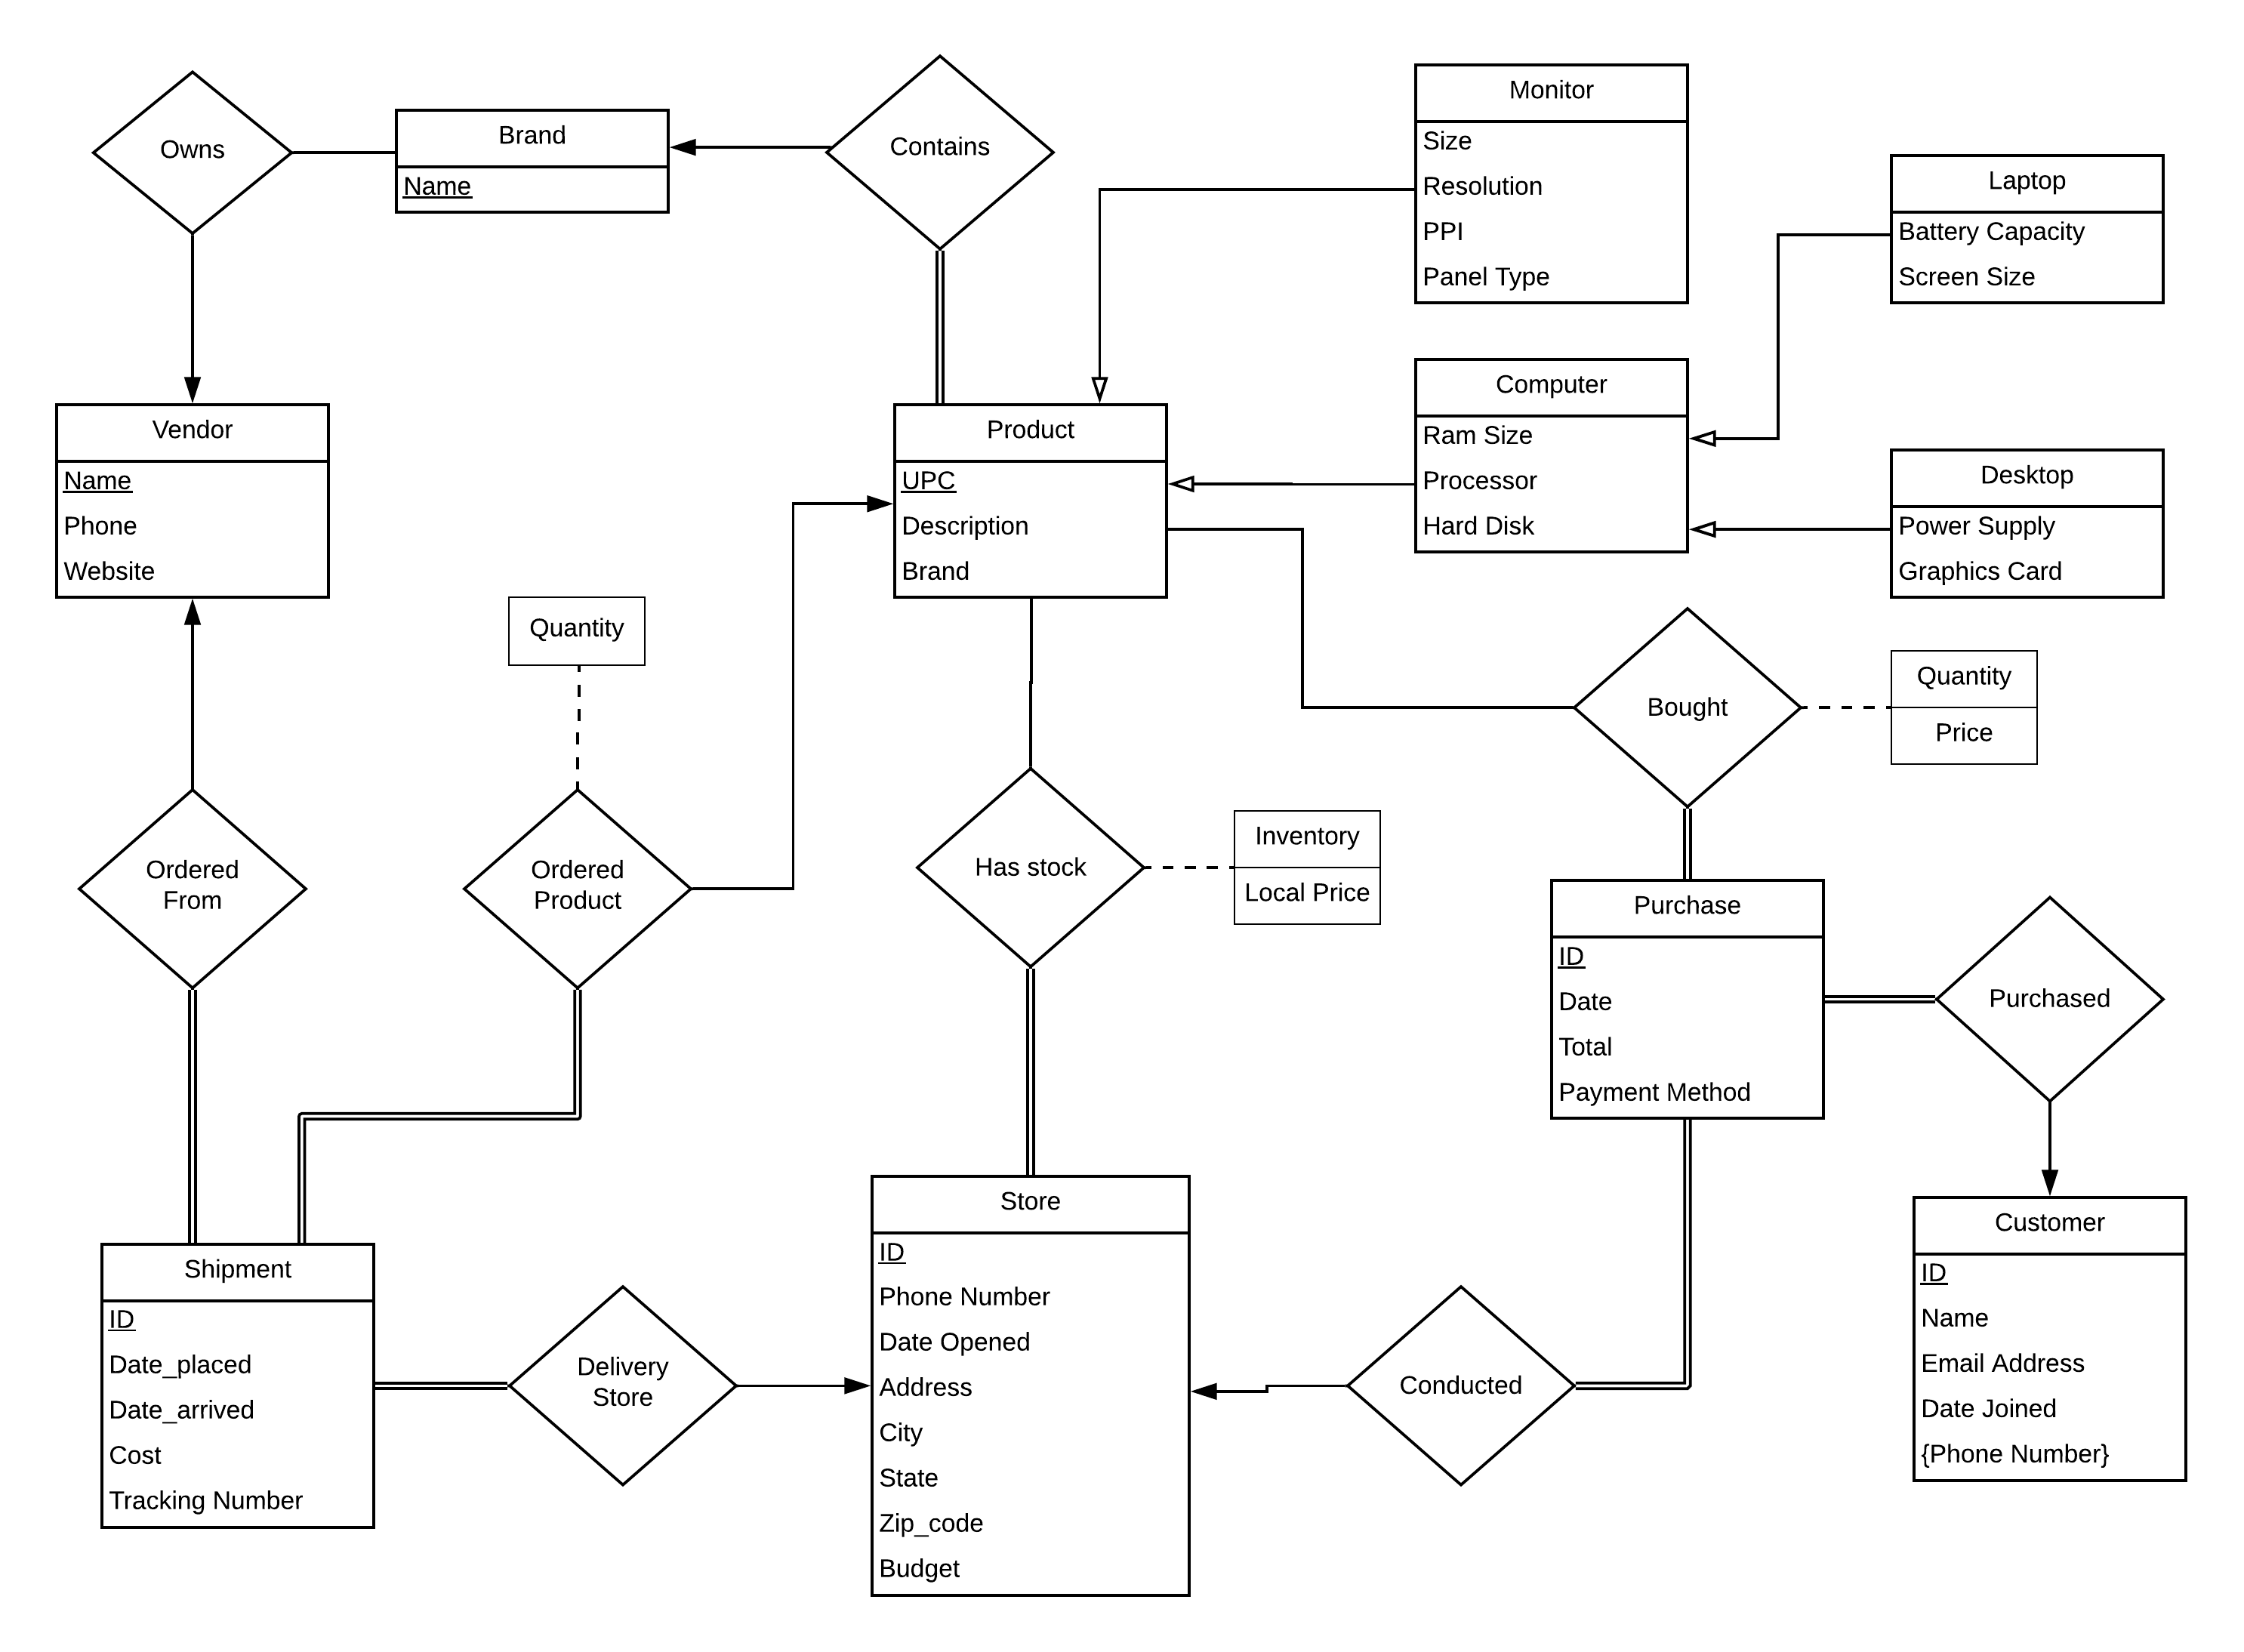
\includegraphics[width=0.95\textwidth]{er_diagram}
      \caption{ER Diagram for Database}
      \label{fig:er}
    \end{figure}

    The Product entity is a major entity in our database. It has a relation with almost every
    entity. This makes sense for a retail database as retailers are generally focused on the
    products they sell. The major products sold at our establishment are Laptops, Desktops,
    Computers, and Monitors. Our product types are Screen and Computer as those make up the two
    major groups of our products. These subgroups inherit identical attributes from parent
    entities. TV obviously inherits from Screen. As the screen is a major component of a
    laptop, laptop also inherits from Screen.  Desktop obviously inherits from Computer,
    however because a laptop is also a computer, it inherits from Computer in addition to
    Screen.

		\noindent 
		The Tables for our database are:
		\begin{itemize}
			\item Product(\underline{UPC}, Description, Brand);
			\item Laptop(\dashuline{UPC}, Battery\_Life, Screen\_Size);
      \item Brand(\underline{Name}, \dashuline{Vendor});
      \item Store(\underline{ID}, Phone\_Number, Date\_Opened, Budget, Address, City, State, Zip\_Code);
			\item Desktop(\dashuline{UPC}, Power\_Supply, Graphics\_Card);
			\item Computer(\dashuline{UPC}, Ram\_Size, Processor, Hard\_Disk);
      \item Monitor(\dashuline{UPC}, Size, Resolution, PPI, Panel\_Type);
			\item Customer(\underline{ID}, Name, Email\_Address, Date\_Joined, Phone\_Number\_1, Phone\_Number\_2);
			\item Vendor(\underline{Name}, Phone, Website);
      \item Shipment(\underline{ID}, Date\_placed, Date\_arrived, Cost, Tracking\_number,
        \dashuline{Vendor\_name}, \dashuline{UPC}, Quantity, \dashuline{Store\_ID});
      \item Purchase(\underline{ID}, Date, Total, Payment\_Method, \dashuline{Customer\_ID}, \dashuline{Store\_ID});
      \item Bought\_Products(\underline{Product\_UPC, Purchase\_ID}, Quantity, Price);
      \item Stock(\underline{Store\_ID, UPC}, Inventory, Listed\_Price);
		\end{itemize}

		\subsection{Products}
      Product contains the attributes UPC and Description. UPC is a unique identifier to
      identify the product in the database. Description is a short description of the product
      for customer and employee benefit. All other attributes associated with a product
      specified by that products subtype.  Our subtypes are Computer and Monitor. All products
      must also have a UPC that matches one in the product above it. For example, a Laptop must
      match a computer that must match a product.

			\subsubsection{Monitor}
				Monitor was chosen as a product type due to our focus on electronics.  A
				large number of electronics these days feature a screen. In addition, the
				monitor is a major consideration in the purchase of an electronic device.

			\subsubsection{Computer}
        Computer is the other major section of the products represented by our database.
        Computer's attributes that are common among all types of computers are RAM size, the
        processor, and the Hard Drive size. 
				\begin{itemize}
          \item Laptop\\
            Laptop inherits from both Computer and Screen because it fits well in both
            categories. All important parts of a Laptop are covered in either Screen or
            Computer, except for Battery Life.
					\item Desktop\\
            A desktop computer is just the tower. It does not include a keyboard, a mouse, or a
            monitor, therefore it does not inherit from Screen. Attributes that apply to
            desktops that don't apply to other computers (Laptops) are the Power Supply, and
            the Graphics Card.
				\end{itemize}

		\subsection{Brand}
			Brand is an alternate way to group products together. The major aspects of
			Brand is the Name and the vendor it belongs to. The Brand names must not 
			match the brand name of any other brand, and the vendor must pair with 
			an existing vendor in the vendor table. 

		\subsection{Vendor}
			A vendor represents a company that our stores purchase products from to
			sell to consumers. A vendor is represented by their company name, their
			phone number, and their website. A vendor is identified by their name as
			that is how they are identified.

		\subsection{Shipment}
			Shipment represents an shipment placed by an employee to resupply a stores
			stock. The shipment consists of a unique ID to identify it, the date it was placed, 
			the date it arrived, the total cost of the shipment, the tracking number for the
			shipment, the vendor name, a UPC, and the quantity, and a store ID. The quantity 
			and UPC are used to keep track of how many of each product was shipment. 
			The vendor name is used to link the shipment with the vendor. The store id is 
			used to keep track of the store the product is being delivered to.

		\subsection{Bought\_Products}
			A table was needed to handle the relation between Purchase and Product
			as multiple of the same product could be purchased in one purchase.
			Price also needed to be tracked as prices of a particular product change
			at different stores.

		\subsection{Store}
			Our database may need to track information about multiple stores. A store
			is represented by a unique ID, the store's phone number, the date the
			store opened, a yearly budget for the store, and the store's address.

		\subsection{Stock}
			A table is needed to manage interactions between Stores and Products.
			A store will sell multiple products, and a product may be stored at
			multiple stores. Stores will have varying inventory of a certain product,
			and may also vary the products type. Stock is represented by a store's
			unique ID, the UPC of a product, how much of that product is currently in
			the store, and the price the store is selling the product for.

		\subsection{Customer}
			Our stores offer a customer loyalty program. This allows customers to be
			tied to the purchases they make. A customer is represented by a unique ID,
			their name, their email address, the date they joined the program, and
			their phone number(s).

		\subsection{Purchase}
			A purchase consists of a unique ID, the date it was placed, the payment
			total, the method of payment (e.g. Credit Card, Debit Card, Cash, etc.), a
			customer ID (e.g. phone number, etc.), and the store ID. A purchase can
			be tied to a customer for the loyalty program. A purchase will not be
			tied to a customer if the customer is not a part of the loyalty program.
			Due to the loyalty program it is likely a customer will be tied to
			multiple purchases, but a single purchase will only be tied to a
			single customer.
			
	\section{Application}
    \begin{figure}[H]
      \centering
      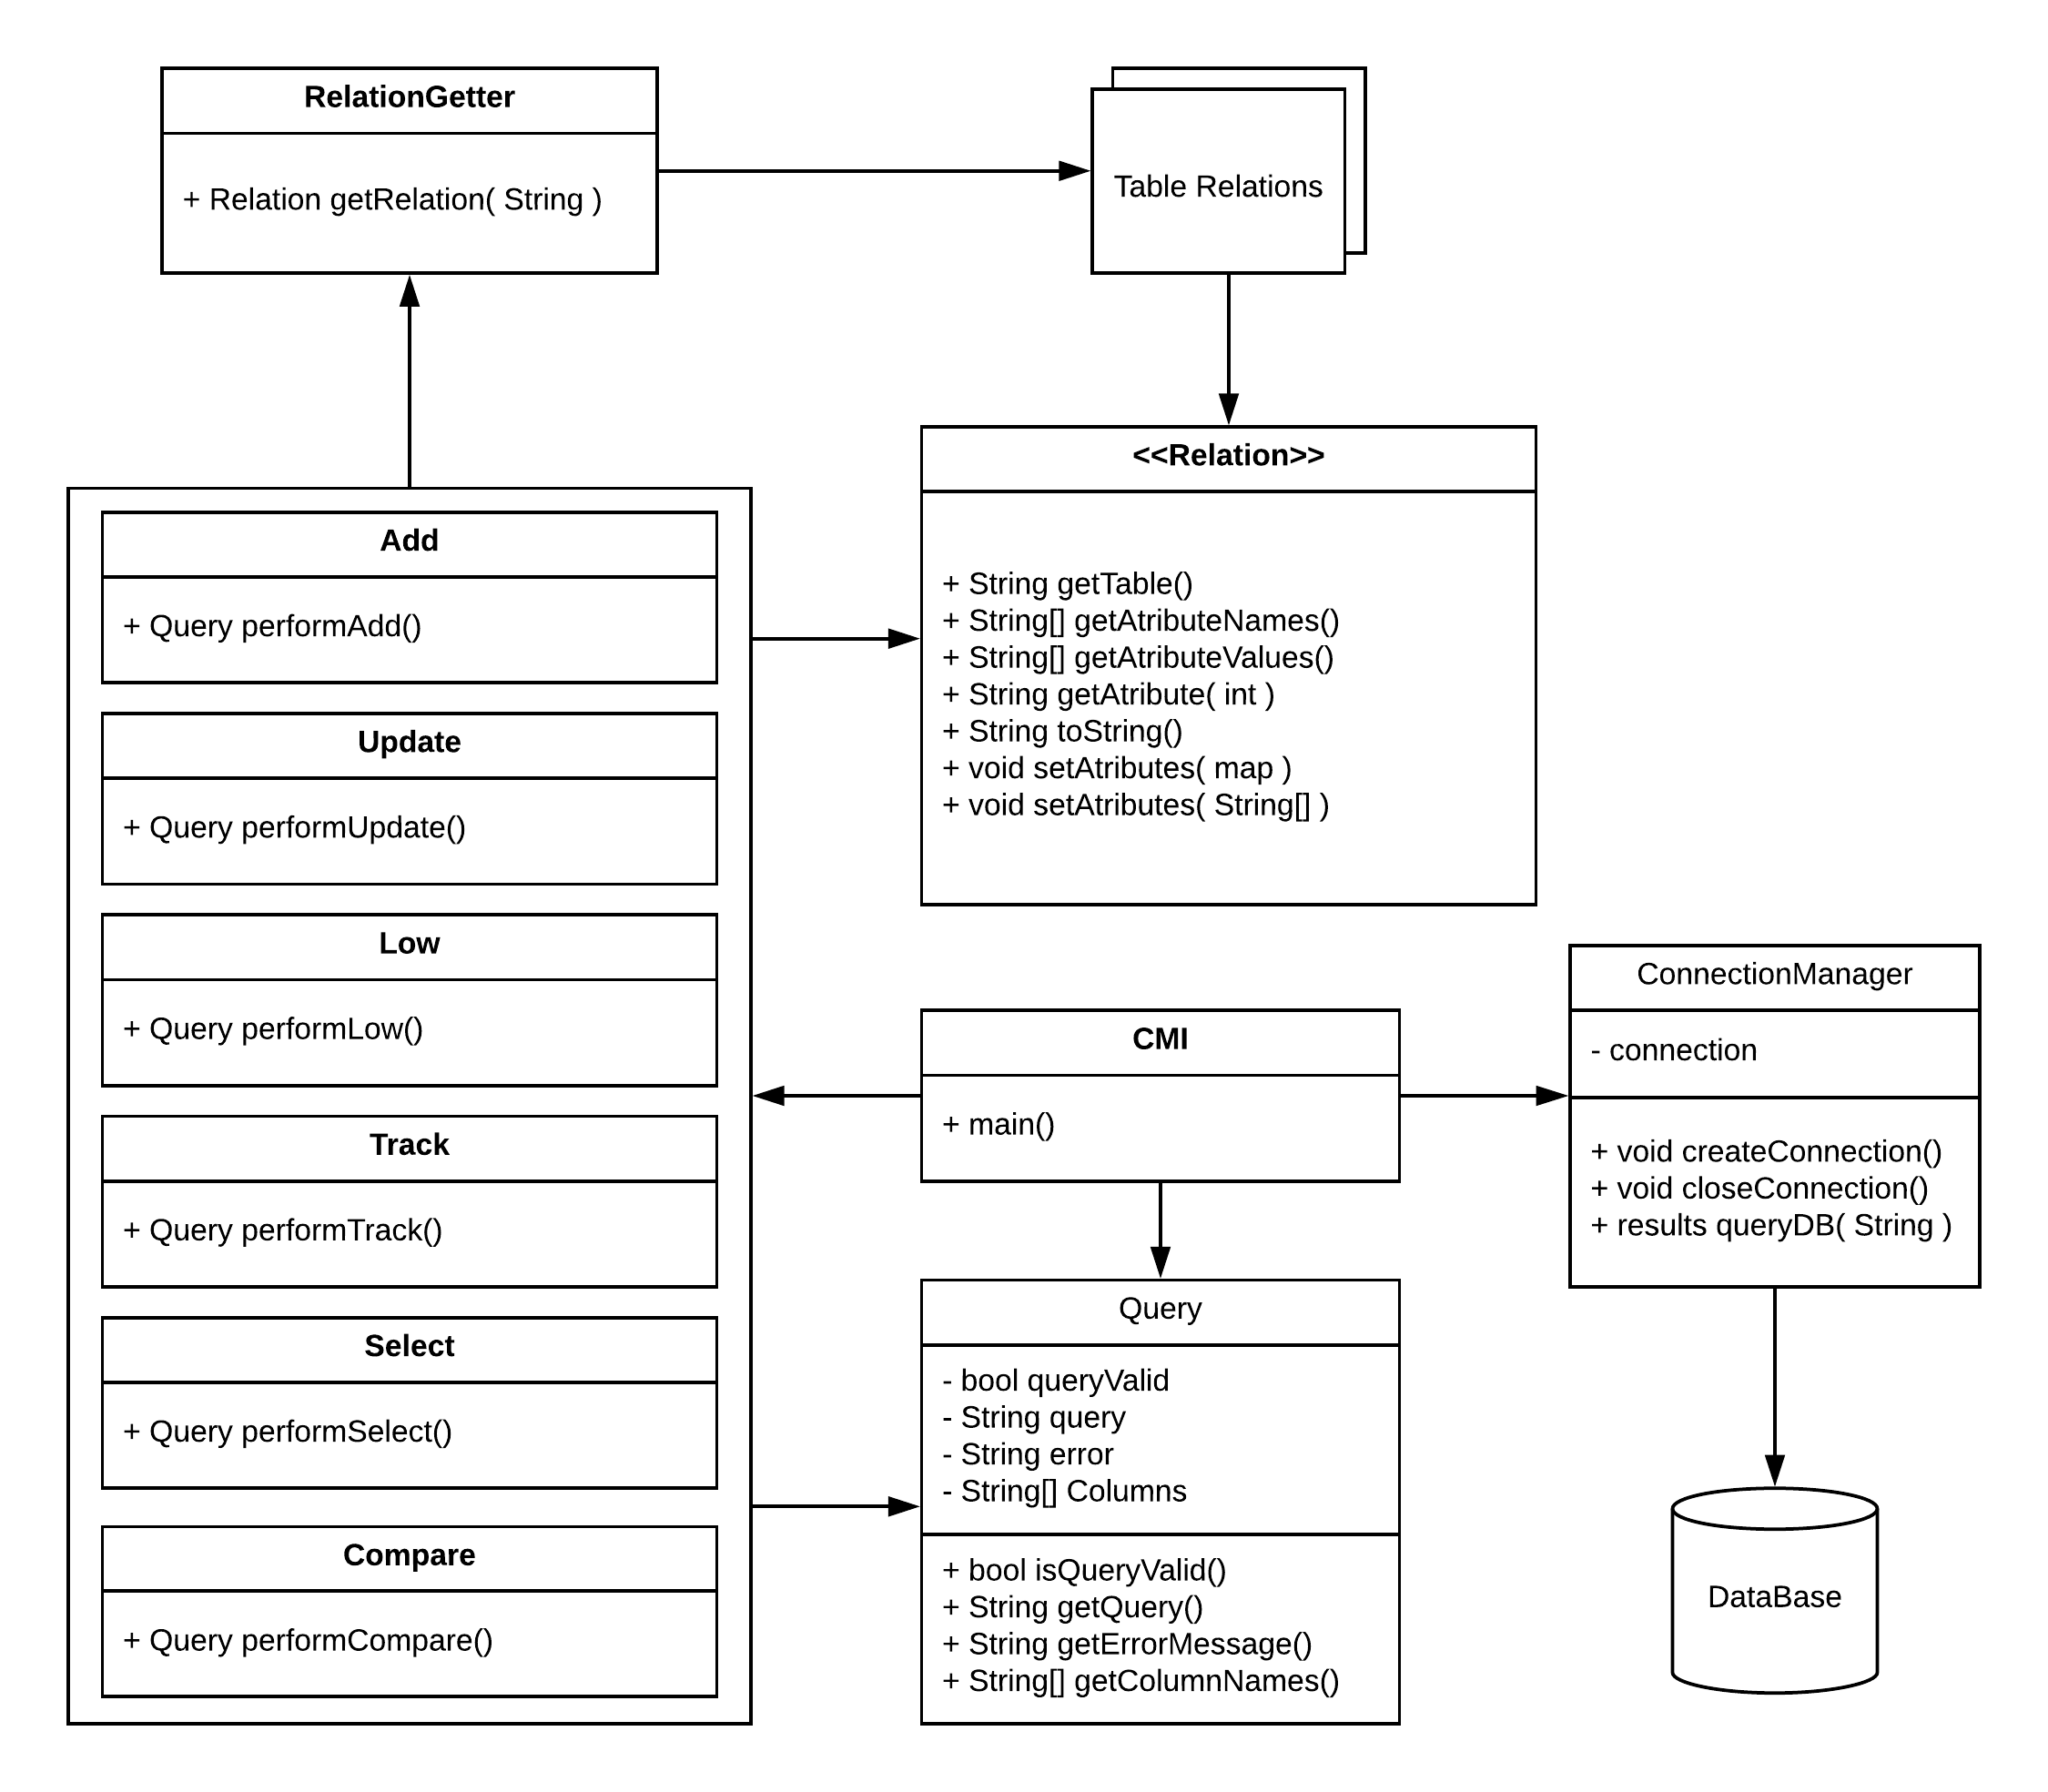
\includegraphics[width=0.85\textwidth]{uml_diagram}
      \caption{UML Diagram for Application}
      \label{fig:uml}
    \end{figure}
	
		\subsection{CMI}
			The CMI handles getting the next command from the user, calling the functions for the specified commands,
			initializing the connections, sending queries to the connection manager and dealing with query results. 
			
		\subsection{ConnectionManager}
			This holds the connection to the database and is the only one to query the database. 
			
		\subsection{Relations}
			Using a relation interface, we will implement a class for every table our project deals with. The relation
			interface will specify functions that will allow getting the values and columns without having to know what
			relation is being used. This allows for creation of generic queries usable with all possible relations.
			
		\subsection{Commands}
			Every command has its own class that generates code based on its specified function (see use cases). 
			They will also get the specified values for the sql using the relation interface to select the requirements
			for its query. It returns a query or an error depending on the values given by the user.
			
		\subsection{RelationGetter}
			Returns a relation object of the type specified. 


	\section{Test Data}
		Our test data was generated to fit the tables made from our ER diagram. The
		data was mostly generated through a random data generator
		(\url{https://www.mockaroo.com/}) and manual construction. Data that was
		independent of other data (such as stores and customers) was generated by
		the random data generator. The rest of the data was generated manually
		and/or through the random data generator to maintain consistency across
		different tables.

	\section{User Interface}
    Our user interface is a command line application using straight forward
    commands. The current commands are as follows.

    \begin{itemize}
      \item
        Add: customer, transaction, store, product, order, vendor, brand\\
        Examples:
        \begin{itemize}
          \item Add customer name=``John Smith" email=john@gmail.com phone=5855551234
          \item Add transaction customer=123 product ``Sony TV 52" 2
        \end{itemize}

      \item
        Update: store, stock, price, customer\\
        Examples:
        \begin{itemize}
          \item Update store 123 phone 1235557890
          \item Update product ``Dell Laptop 15" price=1000 store=123
        \end{itemize}

        \pagebreak

      \item 
        Lowest Inventory:
        \begin{itemize}
          \item Product
          \item Number of low inventory products to show
          \item Sort field: inventory number, expected days until out of stock
          \item Search field: stores
        \end{itemize}
        Examples:
        \begin{itemize}
          \item Low 50 products store=123
          \item Low 5 days store=all
        \end{itemize}

      \item
        Top/Bot: Number of top or bottom records
        \begin{itemize}
          \item Search term: products, product type, stores, brand, vendor
          \item Sort field: revenue, total items sold
          \item Criteria: product type, month/year, store
        \end{itemize}
        Examples:
        \begin{itemize}
          \item Top 5 stores items year=2017
          \item Bot 10 computers revenue store=12
          \item Top 1 brand items product=computer
          \item Top 5 products revenue
        \end{itemize}

      \item
        Compare:
        \begin{itemize}
          \item Comparison of: store, state
          \item Comparison term: brands, products, vendors
          \item Comparison field: revenue, items sold
        \end{itemize}
        Examples:
        \begin{itemize}
          \item Compare stores products laptops computers revenue 
          \item Compare states brands Dell HP items
        \end{itemize}

      \item
        Track: Show items commonly bought together
        \begin{itemize}
          \item Number of records to show
          \item Products, product type
        \end{itemize}
        Examples:
        \begin{itemize}
          \item Track 2 Desktop
        \end{itemize}
    \end{itemize}

  \section{Design Changes}
    A couple design changes were made since Phase 1. The changes are as follows:
    \begin{itemize}
      \item TV was removed
      \item Screen changed to Monitor
      \item Transaction was renamed to Purchase
      \item Order was renamed to Shipment
      \item Order/Shipment was changed to include a store
      \item Store's address was expanded to include City, State, and Zip
    \end{itemize}
    Several changes were made from Phase 1 to improve clarity and simplify the design.  TV was
    removed to reduce the number of tables needed for our design.  Laptop was separated from
    Screen for simplicity. Screen was then changed to Monitor and became a separate product.
    Transaction was renamed to Purchase because transaction is a keyword for SQL.  Order was
    renamed to Shipment because ORDER is an SQL keyword. Shipment was extended to include a
    store so the design could work with multiple stores.  Our design for our UI included the
    ability to query by state. In order for us to know a Store's state, Store's address needed
    to be expanded. Address is now just the street address and Store now includes City, State,
    and Zip Code.
    \subsection{TV and Monitor}


  \end{document}
